\section{Grundlagen der GUI Programmierung}
Apps bestehen aus lose gekoppelten, wiederverwendbaren Komponenten. Diese sind Activities (für den Benutzer sichtbar) und Services, Content Provider, Broadcast Receivers (unsichtbar für Benutzer). \textbf{Erbt nicht von Context und Fragment ist keine Komponente}. Das System hat die Kontrolle über alle Applikationen und Verwaltet den Lebenszyklus, ist verantwortlich für die Kommunikation zwischen Komponenten und schliesst die Apps automatisch um Speicher zu sparen.
\paragraph{Activites} Dies sind die \textbf{Hauptbausteine} in der App Entwicklung, die Activity interagiert mit dem Benutzer. Eine Activity stellt immer auch einen möglichen Eintrittspunkt in die App ein. Bei einem Wechsel in einen anderen Zustand des Lebenszyklus wird die betroffene Activity über einen Methodenaufruf informiert.

\textbf{Activity = Gui + Code}
\begin{lstlisting}[language=java]
public class MainActivity extends Activity {
  @Override
  protected void onCreate(Bundle savedInstanceState) {
    super.onCreate(savedInstanceState);
    /* Hier unser Code z.B
    setContentView(R.layout.activity_main);*/
  }
}
\end{lstlisting}
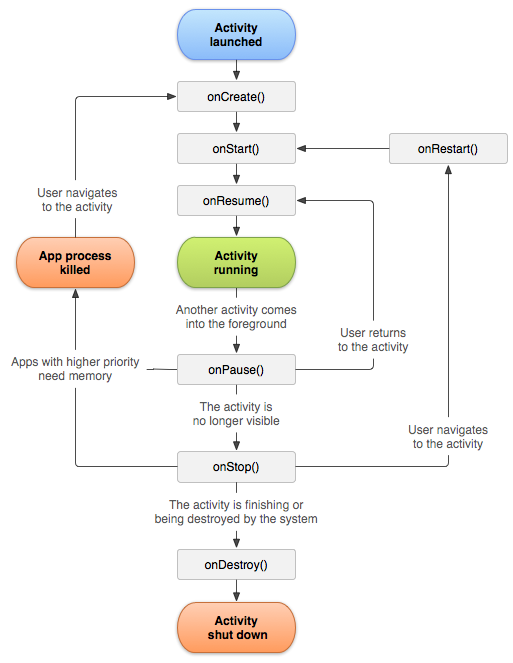
\includegraphics[scale=0.35]{activity_lifecycle.png}
Unterschied Paused/Resume: wird die Activity von einer anderen überdeckt (z.B. Notificationleiste heruntergezogen), wird die erste pausiert (\code{onPause}). Kommt sie wieder in den Vordergrund, wird wieder \code{onResume} aufgerufen.

\code{onPause} ist \textbf{garantiert}. \code{onStop} ist jedoch \textbf{nicht garantiert}. Darum:

\paragraph{Best Practice}

\begin{itemize}
  \item \code{onCreate} erstellt GUI beim Start.
  \item \code{onResume} reagiert auf Benutzereingaben.
  \item \code{onPause} sichert Daten (da die App auch im \code{onStop} oder \code{onDestroy} gekillt werden kann).
  \item \code{onStop} gibt Ressourcen frei.
\end{itemize}

Bei Konfigurationsänderungen wird die Activity neu gestartet. Dazu zählen z.B. \textbf{Screenausrichtungsänderungen}.

\textbf{Stopped/Started:} kommt die Activity wieder in den Vordergrund, weil der User die Applikation nochmal startet oder mit dem Back-Button zurückkommt, wird onRestart() aufgerufen.

\textbf{Destroyed}: die App wird vom System destroyed, oder wenn sie explizit vom User geschlossen wird.

\paragraph{Activity Stack}

Activities werden in einem Stack verwaltet, wobei die Activites eines Stacks zu verschiedenen Apps gehören können.\\ 
Eine \textbf{Gruppe von Activities} in einem Stack nennt man auch \textbf{Task}. Es können mehrere Tasks gleichzeitig existieren. Tasks lassen sich im Overview Screen anzeigen.

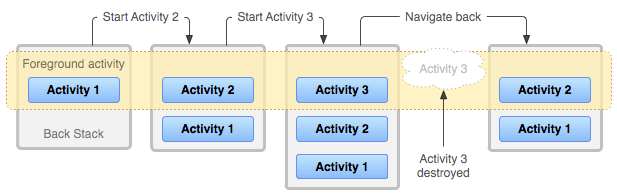
\includegraphics[scale=0.29]{diagram_backstack.png}


\paragraph{APK}

Activities (und Ressourcen, etc) werden in ein APK gepackt und installiert. Wird eine Activity aktiv, wird pro APK ein Linux Prozess mit einem Thread gestartet, welcher alle Activities die indiesem APK enthalten sind ausführt. Jedes APK wird unter einem eigenen Linux-User installiert. Inhalt: Libraries, Ressourcen, Assets, Metadaten, kompilierte Klassen im DEX-Format.

Ein APK ist nichts anderes als ein JAR, welches wiederum eine ZIP-Datei ist.
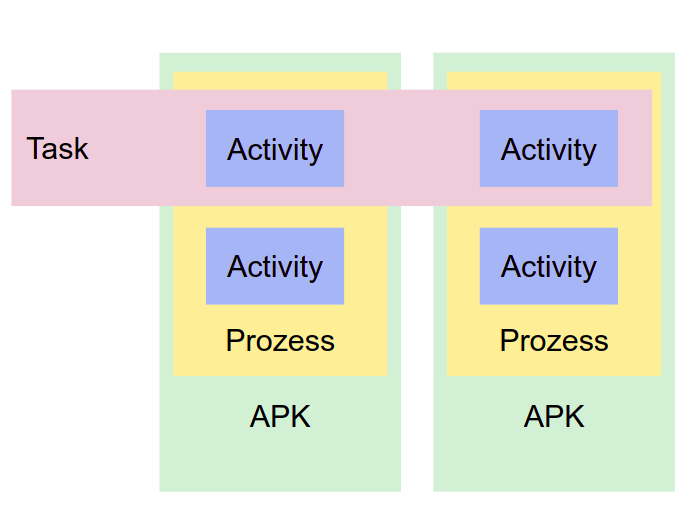
\includegraphics[scale=0.20]{img/activities-tasks-systemsicht.png}

\subsection{Application}
Parent unserer Activities im Manifest ist die Application. Ist auch eine Klasse, die den globalen Zustand unserer App hält. Kann durch eigene Application-Subklasser ersetzt werden. Zugriff aus Activity mit \code{getApplication}, Lifecycle-Methoden: \code{onCreate}, \code{onLowMemory}, \code{onConfigurationChanged}.

\paragraph{Bundle}
Bundles werden in der Regel für den Datenaustausch zwischen verschiedenen Android-Aktivitäten verwendet. Bundles können alle Arten von Werten enthalten und an die neue Aktivität übergeben.

\paragraph{Intent}
\textbf{Kommunikation zwischen Komponenten (Activities, Services, Broadcasts)}
Ein Intent beschreibt was gemacht werden soll \\
- \textbf{Explizit} - Aufruf der Klasse \\
-  \textbf{Implizit} - Aufruf passender Komponente (System entscheidet - geeignet für Systemapps z.B Foto).\\
Apps können selbst wiederum Activites zur Verfügung stellen und bestehende Applikationen ersetzen.
\begin{lstlisting}[language=java]
// Explizit mit Klasse
Intent in = new Intent(this, CalculateActivity.class)
// Implizit mit Aktion z.B Bild erstellen 
Intent in = new Intent(MediaStore.ACTION_IMAGE_CAPUTRE)
\end{lstlisting}
Andere Activities kann man mit \code{startActivity(intent)} oder \code{startActivityForResult(intent, myId)} starten (Resultat wird über Callback kommuniziert und Activity wird nicht blockiert). Um bei letzterem mit dem Rückgabewert arbeiten zu können muss man \code{onActivityResult} überschreiben.
\begin{lstlisting}[language=java]
@Override
protected void onActivityResult(int request, int result, Intent data) {
  if (result == Activity.RESULT_OK && request == myId) {
    /* Resultat verarbeiten */
  }
}
\end{lstlisting}
\begin{lstlisting}[language=java]
//Einfacher Intent aus onCreate Methode
@Override
protected void onCreate(Bundle savedInstanceState) {
    super.onCreate(savedInstanceState);
    setContentView(R.layout.activity_main);

    // einfacher Intent
    final Button button = (Button) findViewById(R.id.btn);
    button.setOnClickListener(new View.OnClickListener() {
        @Override
        public void onClick(View v) {
           Intent it = new Intent(MainActivity.this, SecondActivity.class);
           startActivity(it);
        }
    });
\end{lstlisting}
Möchte man einem Intent Daten übergeben, kann man das entweder mit der \code{setData} Methode, welche eine URI entgegennimmt, oder mit \code{in.putExtra(MediaStore.EXTRA\_OUTPUT, imageCaptureUri)}. Letzere ist eine Struktur mit Key-Value Paaren und nimmt nur primitive Daten, Strings und serialisierbare Datentypen an.
\begin{lstlisting}[language=java]
public class MainActivity extends Activity {

    @Override
    protected void onCreate(Bundle savedInstanceState) {
        super.onCreate(savedInstanceState);
        setContentView(R.layout.activity_main);

        // Intent mit Werten zu arbeiten
        final Button button = (Button) findViewById(R.id.btn);
        button.setOnClickListener(new View.OnClickListener() {
            @Override
            public void onClick(View v) {
               final int myId = 99;
               Intent it = new Intent(MainActivity.this, SecondActivity.class);
               it.putExtra("name", "severin" ); //key value Attribute uebergeben
               startActivityForResult(it, myId); // Activity mit Result starten
            }
        });
    }
    @Override // Activity mit Result auswerten
    protected void onActivityResult(int request, int result, Intent data) {
        if(result == Activity.RESULT_OK && request == 99)
        {
            findViewById(R.id.btn).setEnabled(false);

        }

    }
}

public class SecondActivity extends Activity {

    static final int myId = 99;

    @Override
    protected void onCreate(Bundle savedInstanceState) {
        super.onCreate(savedInstanceState);
        setContentView(R.layout.activity_second);

        TextView txt = findViewById(R.id.txt);
        // Intent Daten/Extras auswerten
        Bundle extras = getIntent().getExtras(); 
        txt.setText(extras.getString("name"));

        final Button button = (Button) findViewById(R.id.btn);
        button.setOnClickListener(new View.OnClickListener() {
            @Override
            public void onClick(View v) {
                // Neuen Intent mit Result erstellen/zurücksenden
                Intent returnIntent = new Intent();
                returnIntent.putExtra("result", "Result OK");
                setResult(Activity.RESULT_OK, returnIntent);
                finish();
            }

        });
    }
}

\end{lstlisting}


\paragraph{Manifest} Das Manifest enthält Meta-Daten einer App. Es umfasst
\begin{itemize}
\item Komponenten der App
\item Metadaten (Name, Icon, Versionsnummer)
\item Permissions (Internet, kostenpflichtige Anrufe etc.)
\item Anforderungen an die Geräte API
\item \code{minSdkVersion} min-Version des Gerätes
\item \code{targetSdkVersion} höchste Version, mit der getestet wurde
\item \textbf{Name der Singleton Instanz der Application (Sub-)Klasse.}
\end{itemize}

Das Manifest wird vom System verwendet um zu wissen, ob die App installiert werden kann, welche Permissions diese verwendet etc.
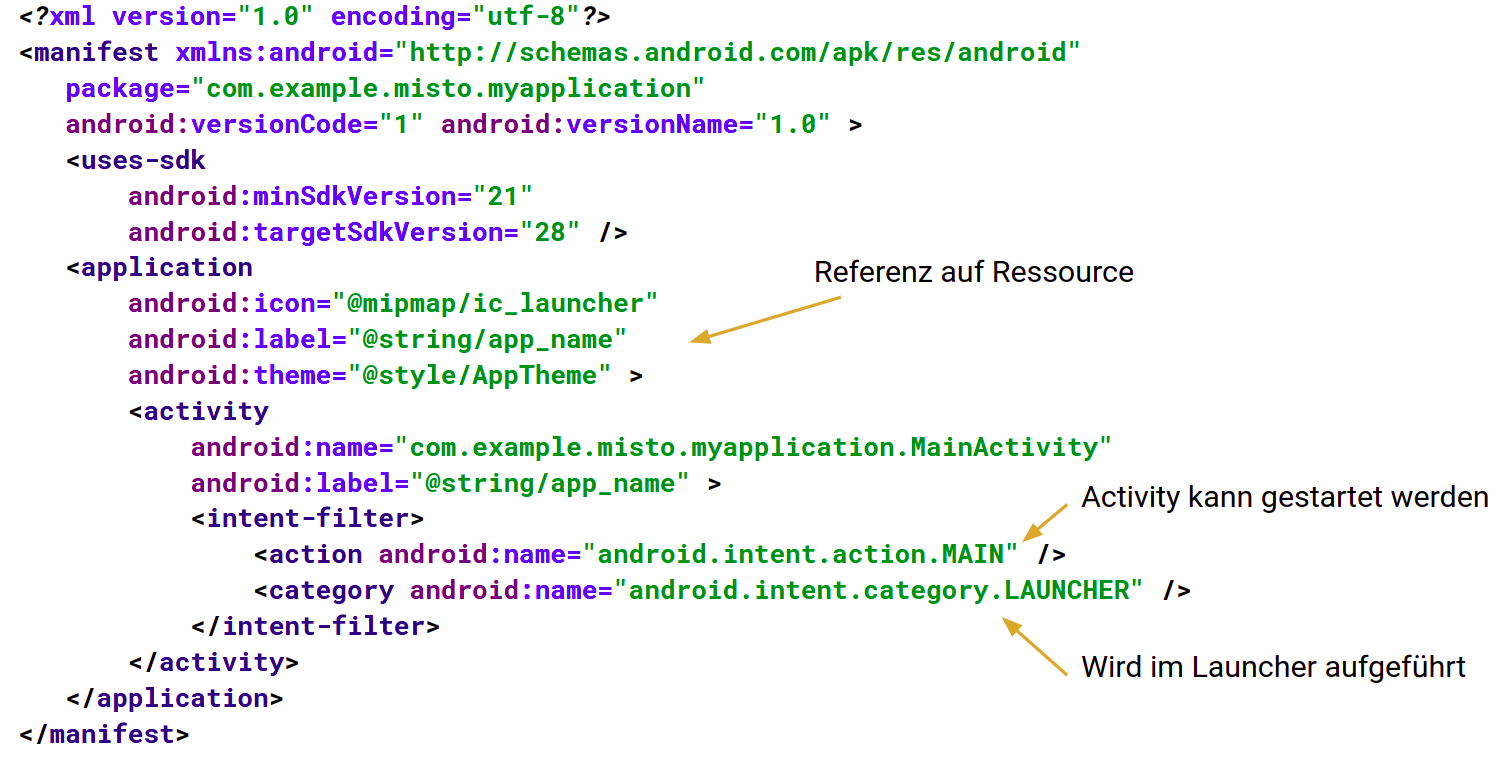
\includegraphics[scale=0.17]{img/manifest.png}

\subsection{Android GUI}
\paragraph{View} Die Basisklasse um User Interfaces zu bauen ist die \code{View}. Eine View ist zuständig seinen Inhalt zu zeichnen und Events zu behandeln. Untergruppen der View sind Widgets und ViewGroups. 
\paragraph{ViewGroup} Die ViewGroup ist eine Unterklasse von View. Sie kann andere View beinhalten. Wenn die ViewGroup beinhaltende View anordnet, spricht man von einem Layout. Composite Design Pattern.
\paragraph{Basis Layout} Layouts sind ViewGroups und beschreiben die visuelle Struktur des UIs.
\includegraphics[scale=0.45]{layouts.png}
Die Layout-Parameter beschreiben wie die Views angeordnet und dargestellt werden. Für alle ViewGroups gemeinsam sind \code{android:layout\_width} und \code{android:layout\_height}. Häufig benutze Werte sind \code{match\_parent} (So gross wie möglich, also wie der Parent erlaubt) und \code{wrap\_content} (so klein wie möglich, also wie die Kinder erlauben).\\

\paragraph{Linear Layout}
In einem \textbf{Linear Layout} werden die Elemente horizontal oder vertikal angeordnet. Mit \code{android:layout\_weight} kann man Elementen ein Gewicht geben, da es selten sinnvoll ist, alle Elemente gleich gross zu lassen. Kinder ohne Weight bekommen minimalen Platz, auf die restlichen wird der verfügbare Platz nach Gewicht aufgeteilt.\\ 
\begin{lstlisting}[language=xml]
<LinearLayout 
 android:layout_width="match_parent"
 android:layout_height="match_parent"
 android:orientation="vertical">
 <TextView
    android:layout_width="match_parent"
    android:layout_height="wrap_content"
    android:textAlignment="center"
    android:background="@color/colorPrimaryDark"
    android:textColor="#FFFFFF"
    android:text="eins"/>
 <TextView
    android:layout_width="match_parent"
    android:layout_height="wrap_content"
    android:textAlignment="center"
    android:text="zwei"/>
 <TextView
    android:layout_width="match_parent"
    android:layout_height="wrap_content"
    android:textAlignment="center"
    android:background="@color/colorPrimaryDark"
    android:textColor="#FFFFFF"
    android:text="drei"/>
</LinearLayout>
\end{lstlisting}
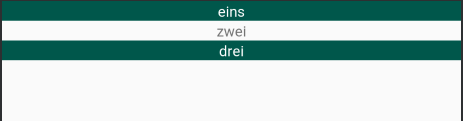
\includegraphics[scale=0.3]{img/linearlayout_1.png} 

\begin{lstlisting}[language=xml]
<LinearLayout 
    android:layout_width="match_parent"
    android:layout_height="match_parent"
    android:orientation="vertical">
    <TextView
        android:layout_width="match_parent"
        android:layout_weight="1"
        android:textAlignment="center"
        android:background="@color/colorPrimaryDark"
        android:textColor="#FFFFFF"
        android:text="eins"/>
    <TextView
        android:layout_width="match_parent"
        android:layout_weight="1"
        android:textAlignment="center"
        android:text="zwei"/>
    <TextView
        android:layout_width="match_parent"
        android:layout_weight="1"
        android:textAlignment="center"
        android:background="@color/colorPrimaryDark"
        android:textColor="#FFFFFF"
        android:text="drei"/>
</LinearLayout>
\end{lstlisting}
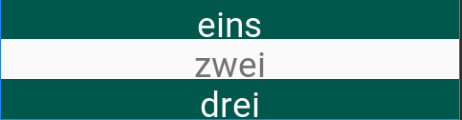
\includegraphics[scale=0.3]{img/linearlayout_2.png} 

\begin{lstlisting}[language=xml]
<LinearLayout 
 android:layout_width="match_parent"
 android:layout_height="match_parent"
 android:orientation="vertical">
 <TextView
    android:layout_width="match_parent"
    android:layout_height="wrap_content"
    android:layout_weight="0"
    android:textAlignment="center"
    android:background="@color/colorPrimaryDark"
    android:textColor="#FFFFFF"
    android:text="eins"/>
 <TextView
    android:layout_width="match_parent"
    android:layout_height="wrap_content"
    android:layout_weight="1"
    android:textAlignment="center"
    android:text="zwei"/>
 <TextView
    android:layout_width="match_parent"
    android:layout_height="wrap_content"
    android:layout_weight="0"
    android:textAlignment="center"
    android:background="@color/colorPrimaryDark"
    android:textColor="#FFFFFF"
    android:text="drei"/>
</LinearLayout>
\end{lstlisting}
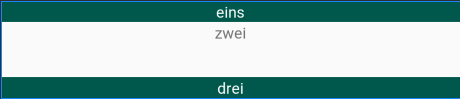
\includegraphics[scale=0.3]{img/linearlayout_3.png} 

\paragraph{Relative Layout}
\begin{lstlisting}[language=xml]
<RelativeLayout
 android:layout_width="match_parent"
 android:layout_height="match_parent">
 <TextView
    android:id="@+id/center"
    android:layout_width="wrap_content"
    android:layout_height="wrap_content"
    android:layout_centerInParent="true"
    android:text="Center"/>
 <TextView
    android:layout_width="wrap_content"
    android:layout_height="wrap_content"
    android:layout_toLeftOf="@id/center"
    android:layout_alignBottom="@id/center"
    android:text="2"/>
 <TextView
    android:layout_width="wrap_content"
    android:layout_height="wrap_content"
    android:layout_toRightOf="@id/center"
    android:layout_alignBottom="@id/center"
    android:text="3"/>
 <TextView
    android:layout_width="wrap_content"
    android:layout_height="wrap_content"
    android:layout_above="@id/center"
    android:layout_alignLeft="@id/center"
    android:text="1"/>
 <TextView
    android:layout_width="wrap_content"
    android:layout_height="wrap_content"
    android:layout_below="@id/center"
    android:layout_alignLeft="@id/center"
    android:text="4"/>
</RelativeLayout>
\end{lstlisting}
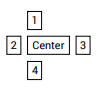
\includegraphics[scale=0.7]{relativelayout.png} \\
\textbf{Beispiele verstehen:} \\
Linke Kante ausrichten auf Linke Kante von ID-Element: \code{android:layout\_alignLeft} \\
Linke Kante ausrichten auf Rechte Kante von ID-Element: \code{android:layout\_toRightOf}\\
Unten/Oben ausrichten: \code{android:layout\_above | android:layout\_below}\\
Ausrichten am Parent: \code{android:layout\_centerInParent="true" | android:layout\_alignParentBottom="true"} etc. \\
\code{android:layout\_alignBaseline} um Text auf gleiche Höhe zu bringen (ohne Margin)
\paragraph{Weitere Layouts}
\begin{itemize}
  \item Frame Layout: Kinder übereinander anordnen (Linien bei einer Kamera App). In Activity Klasse mit \code{setContentView(R.layout.activity\_main)}
  \item FlexboxLayout: CSS Flexbox
  \item ConstraintLayout, mit RelativeLayout verwandt (war in Android Studio immer Standard ab irgendeiner Version)
  \item WebView um HTML anzuzeigen: JavaScript kann aktiviert werden, und Java-Objekte können mit JS angesprochen werden
\end{itemize}

\subsection{View setzen und GUI-Objekt finden finden}
\begin{lstlisting}[language=java]
//View Setzen
setContentView(R.layout.activity_main);
//View/Elemente finden
Button button = (Button) findViewById(R.id.button)
\end{lstlisting}
findViewById innerhalb einer Activity sucht im aktuellen Layout (wahrscheinlich dasjenige von \code{setContentView}). Rückgabe ist immer die Oberklasse \code{View},  das Resultat muss also noch gecastet werden.

Hat man allerdings ein Fragment oder z.B. ein Listenelement, so muss man die Parent-View vorher gespeichert haben (z.B. die Rückgabe des \code{LayoutInflater}), und dann auf dieser die gewünschte View finden. 

\subsection{Widgets}
Widgets ist ein Sammelbegriff für alle fix-fertigen Komponenten für User-Interfaces (Buttons, Images, Checkboxes etc.)

\paragraph{Button}
\begin{lstlisting}[language=xml]
<Button
    android:layout_width="wrap_content"
    android:layout_height="wrap_content"
    android:text="Alarm"
    android:id="@+id/alarmButton" />
\end{lstlisting}
Bei \code{<ImageButton/>} kann das Bild mit \code{android:src="..."} geladen werden.
\paragraph{Eingabefelder}
\begin{lstlisting}[language=xml]
<EditText
android:id="@+id/phone"
android:layout_width="match_parent"
android:layout_height="wrap_content"
android:inputType="phone|textCapSentences|textAutoCorrect" />
\end{lstlisting}
\paragraph{Referenzen und ID}
\begin{lstlisting}[language=java]
// ID setzen
android:id="@+id/id_name
// ID referenzieren 
android:layout_below="@id/id_name"
\end{lstlisting}
Die Klasse R enthält alle IDs und Ressourcen( Layoutdateien, drawable[Bilder], menu[Menüs], mipmap[Launcher Icon der App], values[strings, etc.]) als Konstanten. 
\paragraph{Ressourcen} Konstanten in \code{dimens.xml} werden für Grössen in den Layouts benutzt.
Die Ordnernamen müssen in Java-Namen umgewandelt werden können, dürfen also z.B. kein \code{-} enthalten. Gleiches gilt auch für  \code{strings.xml}. Zugriff mit  \code{getString(R.string.app\_name);} 

\begin{lstlisting}[language=xml]
<!-- Layout -->
<RelativeLayout xmlns:android="..." xmlns:tools="..."
  android:layout_width="match_parent"
  android:layout_height="match_parent"
  android:paddingLeft="@dimen/activity_horizontal_margin"
  android:paddingRight="@dimen/activity_horizontal_margin"
  android:paddingTop="@dimen/activity_vertical_margin"
  android:paddingBottom="@dimen/activity_vertical_margin"
  tools:context=".MainActivity">
<!-- dimens.xml -->
  <!-- Default screen margins, per the Android Design guidelines. -->
  <dimen name="activity_horizontal_margin">16dp</dimen>
  <dimen name="activity_vertical_margin">16dp</dimen>
</resources>
\end{lstlisting}
Grössenangeben von Views erfolgen in density-indepentent Pixels (dp oder dip). Bei Schriften verwendet man scale-independent Pixels (sp).
\paragraph{Events und Event Handling}\label{grundlagen:eventhandling} Das Android-Framework hat einen sogenannten Event-Loop (Looper). Dieser wartet bis ein Ereignis passiert und verarbeitet dieses dann. \textbf{Nur der Main-Thread darf das GUI verändern.} \\
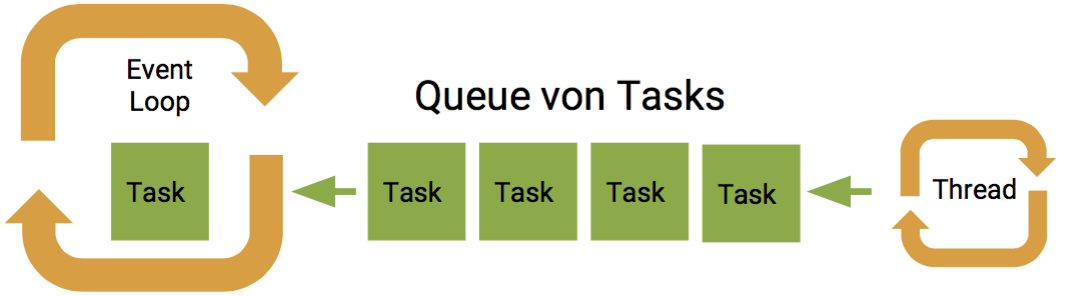
\includegraphics[scale=0.25]{EventLoops.png} \\

\paragraph{Event Listener}
Fast alle Listener können mit \code{set[EventName]Listener} registriert werden.
\begin{itemize}
    \item OnTouchListener: Touch Events
    \item OnClickListener: Wenn View angegklickt wird
    \item OnLongClickListener: touch and hold einer View
    \item OnKeyListener: wenn Hardware Taste ausgelöst wird.
\end{itemize}
\begin{lstlisting}[language=java]
button.setOnClickListener(new View.OnClickListener() {
  @Override
  public void onClick(View v) {
    /* ... */
  }
});
//oder direkt mit einem Lambda:
button.setOnClickListener( v -> { /* ... */ }); 
\end{lstlisting}
Oder onClick Listener in XML deklariert
 \begin{lstlisting}[language=java]
 // im xml:
 android:onClick="onButtonClicked"
 // onButtonClicked im Java implementieren
 public void onButtonClicked(View view) { /*....*/}
 \end{lstlisting}

Ein Listener lässt sich auch bei mehreren Views registrieren.
\begin{lstlisting}[language=java]
public void onClick(View view) {
    if (view == btn1) { // Code für btn1
    } else if (view == btn2) { // Code für btn2
}}
\end{lstlisting}

\paragraph{TextWatcher}
\begin{itemize}
\item \code{beforeTextChanged}: Wird aufgerufen bevor der Text geändert wird
\item \code{onTextChanged}: Wird aufgerufen sobald der Text geändert hat
\item \code{afterTextChanged}: Nachdem der Text geändert wurde, kann man den Text noch anpassen (Loop-Gefahr)
\end{itemize}
\begin{lstlisting}[language=java]
editText.addTextChangedListener(new TextWatcher() {
  public void onTextChanged(CharSequence s, int start, int before, int count){ }
  public void beforeTextChanged(CharSequence s, int start, int count, int after){ }
  public void afterTextChanged(Editable s) { }
});
\end{lstlisting}
\textbf{Inputvalidierung:}
\begin{lstlisting}[language=java]
final EditText password = (EditText) findViewById(R.id.password);
password.addTextChangedListener(new TextWatcher() {
  @Override
  public void afterTextChanged(Editable s) {
    String pw = s.toString();
    if (s.length() < 8) {
    password.setError("Passwort muss mindestens 8 Zeichen lang sein.");
    }
  }
  ...
});
\end{lstlisting}
%\subsection{Android Testing mit JUnit}
%Es gibt mehrere Arten von Tests für eine Activity. Die \code{ActivityUnitTest} manipulieren das UI im Code, die \code{ActivityInstrumentationTestCase2} schickt Clicks und Events an das UI. Um eine App mit mehreren Activities zu testen, gibt es das Espresso Framework, sowie UI Automator um App-übergreifend zu testen.
%\begin{lstlisting}[language=java]
%public class MainActivityLayoutTest extends ActivityUnitTestCase<MainActivity> {
%  public MainActivityLayoutTest() {
%    super(MainActivity.class);
%  }
%  @Override
%  protected void setUp() throws Exception {
%    super.setUp();
%    ContextThemeWrapper context = new
%      ContextThemeWrapper(getInstrumentation().getTargetContext(), R.style.AppTheme);
%    setActivityContext(context);
%    startActivity(
%      new Intent(getInstrumentation().getTargetContext(), MainActivity.class),null,null);
%}
%\end{lstlisting}
%Funktionale Tests (ActivityInstrumentationTestCase2) testen eine Activity im echten Systemkontext. Der Test löst Events aus und prüft, ob diese zum erwünschten Resultat führen. Dazu gehören: 
%\begin{itemize}
%\item Ändert sich das UI wie erwartet
%\item Überprüfen von Inputvalidierung
%\item Werden Lifecycle Events korrekt behandelt
%\end{itemize}
%\begin{lstlisting}[language=java]
%public class MainActivityInteractionTest extends ActivityInstrumentationTestCase2<MainActivity> {
%  public MainActivityInteractionTest() { super(MainActivity.class); }
%  public void testSayHi() {
%    MainActivity activity = getActivity();
%    final EditText editText = (EditText) activity.findViewById(R.id.editText);
%    getInstrumentation().runOnMainSync(new Runnable() {
%      @Override
%      public void run() {
%        editText.requestFocus();
%      }
%    });
%    getInstrumentation().waitForIdleSync();
%    getInstrumentation().sendStringSync("Hello");
%    getInstrumentation().waitForIdleSync();
%    Button button = (Button) activity.findViewById(R.id.button);
%    TouchUtils.clickView(this, button);
%...
%\end{lstlisting}
